



\section{The Standard Multi-Player Performative Prediction Form}
\label{Appendix:refumulation}
In this section, we rewrite our problem in the multi-player performative prediction form given in \cite{narang2023multiplayer}.  Let: 
\begin{itemize}
    \item \(p(y)\): the probability density function of the credit score \(y\) under \(D_y\).
    \item \(g_1(\theta_1, \theta_2, y) = (1 + \gamma_1)y - (1 - y)\): the expected reward of Bank 1 for a customer with score \(y\) (if the customer chooses Bank 1).
    \item \(D_{1, \theta_1, \theta_2}\): the distribution of credit score \(y\) for customers choosing Bank 1, given strategies \(\theta_1\) and \(\theta_2\).
\end{itemize}

The p.d.f. of \(D_{1, \theta_1, \theta_2}\), denoted \(p_1(\theta_1, \theta_2, y)\), is:
\[
p_1(\theta_1, \theta_2, y) =  
\begin{cases}
0,  & y < \tau_1 \text{ or } (\tau_1, \tau_2 \leq y \text{ and } \gamma_1 > \gamma_2);    \\
\frac{p(y)}{Z_1(\theta_1, \theta_2)},   & \tau_1 \leq y < \tau_2 \text{ or } (\tau_1, \tau_2 \leq y \text{ and } \gamma_1 < \gamma_2); \\
\frac{p(y)}{2Z_1(\theta_1, \theta_2)}, & \tau_1, \tau_2 \leq y \text{ and } \gamma_1 = \gamma_2,             \\
\end{cases}
\]
where \(Z_1(\theta_1, \theta_2)\) is the normalization constant:
\[
Z_1(\theta_1, \theta_2) = 
\begin{cases}
\int_{\tau_1}^1 p(y) \, dy,  & \text{if } \gamma_1 < \gamma_2; \\
\frac{1}{2} \int_{\tau_1}^1 p(y) \, dy,  & \text{if } \gamma_1 = \gamma_2; \\
\int_{\tau_1}^{\tau_2} p(y) \, dy, & \text{if } \gamma_1 > \gamma_2.
\end{cases}
\]

Using this, the utility function for Bank 1 can be rewritten as:
\[
u_1(\theta_1, \theta_2) = \mathbb{E}_{y \sim D_{1, \theta_1, \theta_2}} \big[g_1(\theta_1, \theta_2, y) Z_1(\theta_1, \theta_2)\big].
\]

In this performative prediction framework, the distribution \(D_{1,\theta_1,\theta_2}\) depends discontinuously on the strategies \(\theta_1\) and \(\theta_2\), making it non-Lipschitz. This characteristic highlights the distinctiveness of the model compared to standard performative prediction problems.


\section{Property of the $f$ function} 
We first introduce the following simple lemma about the properties of $f$, which is easy to check based on the definition given in \eqref{eqn:utility-onebank}.
\begin{lemma}
\label{lem:property of f}
Assume $\emph{Supp}(D_y)=[0,1]$. We have the following:
\begin{enumerate}
\item Let $\tau_a<\tau_b<\tau_c$. Then $f_{D_y}(\gamma_1,\tau_a,\tau_c)=f_{D_y}(\gamma_1,\tau_a,\tau_b)+f_{D_y}(\gamma_1,\tau_b,\tau_c)$.
    \item $f(\gamma,\tau_a,\tau_b)$ is monotonically increasing with respect to $\gamma$. 
     \item We have $f(\gamma,\tau_a,\tau_b)\in[-1,2]$. 
    \item Let $y_{\gamma}=\frac{1}{2+\gamma}$. If $y_{\gamma}\in(\tau_a,\tau_b)$, then $f(\gamma,\tau_a,y_{\gamma})<0$, and  $f(\gamma,y_{\gamma},\tau_b)>0$.    
\end{enumerate}   
\end{lemma}
\begin{proof}
    We first recall the definition of $f$: 
    \begin{equation*}
    f_{D_y}(\gamma,\tau_a,\tau_b)=\int_{\tau_a}^{\tau_b}[(2+\gamma)y-1]p(y)dy.
\end{equation*}
The first property can be easily obtained based on the integration form. For the second property, it can be seen that for any $\delta>0$, 
$$f(\gamma+\delta,\tau_{a},\tau_b)=f(\gamma,\tau_{a},\tau_b)+ \int_{\tau_{a}}^{\tau_b}\delta yp(y)dy> f(\gamma,\tau_{a},\tau_b).$$
For the third property, we have 
$$ -1=\min_{y\in[0,1]}(2+\gamma)y-1\leq f(\gamma,\tau_{a},\tau_b)\leq \max_{y\in[0,1]}(2+\gamma)y-1\leq 2. $$
For the last property, it can be proved by noticing that $(2+\gamma)y_{\gamma}-1=0$.
\end{proof}
%\noindent We analyze the existence of pure Nash equilibria under different conditions on the relationship between  decision pairs $\theta_1,\theta_2$. Firstly, note that, for a pair of $\theta_1,\theta_2$,  if the utility of a bank is strictly less than $0$, then the bank can always adjust its parameters $\gamma$ and $\tau$ to $1$ to ensure its utility becomes non-negative. This implies that decision pairs leading to non-positive utilities will not be an Nash equilibrium. Therefore, we only need to consider cases where $u_1 \geq 0$ and $u_2 \geq 0$. 

\section{Proofs for Section \ref{sec:understand NE}: Equilibrium Characterization}
In this section, we provide the proof of the conclusions given in Section \ref{sec:understand NE}.


\subsection{Proof of Theorem \ref{thm:pureNE}}
\label{proof:Theorem:pure:NE}
Since the utility matrix of this problem can be represented as a \(4 \times 4\) matrix, the pure Nash equilibria (NE) can be obtained by analyzing the asymmetric best response dynamics. Consider a dynamic process where Banks 1 and 2 alternately update their strategies by playing their best responses, conditioned on observing the opponent's decisions. Based on different initializations (all four decisions) for Bank 2, we obtain the results shown in Figure \ref{fig:enter-label} under various conditions. The figure clearly illustrates the pure Nash equilibria for different scenarios.


\begin{figure}[H]
    \centering
\resizebox{0.47\textwidth}{!}{    
\fbox{
\begin{minipage}{0.5\textwidth}
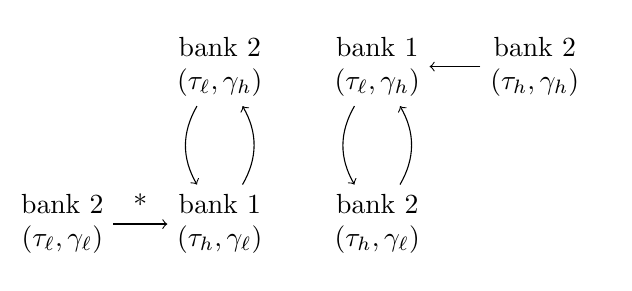
\begin{tikzpicture}
  % Nodes
    \hspace{-0.2cm}\node[align=center] (A) at (-2,0) {bank 2 \\ $(\tau_{\ell},\gamma_{\ell})$};
  \node[align=center] (B) at (0,0) {bank 1 \\ $(\tau_{h},\gamma_{\ell})$};
  \node[align=center] (C) at (2,0) {bank 2\\ $(\tau_{h},\gamma_{\ell})$};
  \node[align=center] (D) at (0,2) {bank 2\\ $(\tau_{\ell},\gamma_{h})$};
  \node[align=center] (E) at (2,2) {bank 1  \\ $(\tau_{\ell},\gamma_{h})$};
  \node[align=center] (F) at (4,2) {bank 2 \\ $(\tau_{h},\gamma_{h})$};
  % Arrows
  \draw[->] (A) -- node[above]{*} (B);
  %\draw[->,red] (D) -- (E);
  %\draw[->,red] (C) -- (B);
  %\draw[->,red] (F) -- (C);
  \draw[->,bend right] (B) to (D);
  \draw[->,bend right] (D) to (B);
  \draw[->,bend right] (E) to (C);
    \draw[->,bend right] (C) to (E);
    \draw[->] (F) to (E);
\end{tikzpicture} 
\caption{$\epsilon_1<0, \epsilon_2>0$.}
\end{minipage}
}
}
\resizebox{0.47\textwidth}{!}{    
\fbox{
\begin{minipage}{0.50\textwidth}
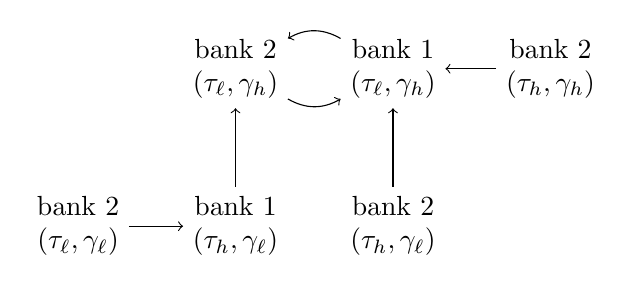
\begin{tikzpicture}
  % Nodes
    \node[align=center] (A) at (-2,0) {bank 2 \\ $(\tau_{\ell},\gamma_{\ell})$};
  \node[align=center] (B) at (0,0) {bank 1 \\ $(\tau_{h},\gamma_{\ell})$};
  \node[align=center] (C) at (2,0) {bank 2\\ $(\tau_{h},\gamma_{\ell})$};
  \node[align=center] (D) at (0,2) {bank 2\\ $(\tau_{\ell},\gamma_{h})$};
  \node[align=center] (E) at (2,2) {bank 1  \\ $(\tau_{\ell},\gamma_{h})$};
  \node[align=center] (F) at (4,2) {bank 2 \\ $(\tau_{h},\gamma_{h})$};
  % Arrows
  \draw[->] (A) -- (B);
  %\draw[->,red] (D) -- (E);
  %\draw[->,red] (C) -- (B);
  %\draw[->,red] (F) -- (C);
  \draw[->] (B) to (D);
  \draw[->] (C) to (E);
  \draw[->,bend right] (D) to (E);
    \draw[->,bend right] (E) to (D);
    \draw[->] (F) to (E);
\end{tikzpicture} 
\caption{$\epsilon_1>0, \epsilon_2>0$.}
\end{minipage}
}
}
\resizebox{0.47\textwidth}{!}{ 
\fbox{
\begin{minipage}{0.5\textwidth}
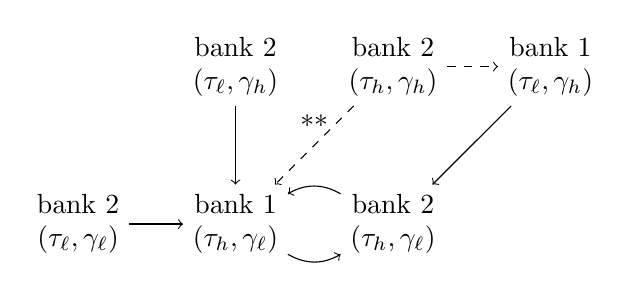
\begin{tikzpicture}
  % Nodes
    \node[align=center] (A) at (-2,0) {bank 2 \\ $(\tau_{\ell},\gamma_{\ell})$};
  \node[align=center] (B) at (0,0) {bank 1 \\ $(\tau_{h},\gamma_{\ell})$};
  \node[align=center] (C) at (2,0) {bank 2\\ $(\tau_{h},\gamma_{\ell})$};
  \node[align=center] (D) at (0,2) {bank 2\\ $(\tau_{\ell},\gamma_{h})$};
  \node[align=center] (E) at (2,2) {bank 2  \\ $(\tau_{h},\gamma_{h})$};
  \node[align=center] (F) at (4,2) {bank 1 \\ $(\tau_{\ell},\gamma_{h})$};
  % Arrows
  \draw[->] (A) -- (B);
  \draw[->] (F) -- (C);
  %\draw[->,red] (D) -- (E);
  %\draw[->,red] (C) -- (B);
  %\draw[->,red] (F) -- (C);
  \draw[->,dashed] (E) -- node[above]{**} (B);
  \draw[->,dashed] (E) -- (F);
  \draw[->] (D) to (B);
  \draw[->,bend right] (B) to (C);
    \draw[->,bend right] (C) to (B);
\end{tikzpicture} 
\caption{$\epsilon_1<0,\epsilon_2<0$.}
\end{minipage}
}
}
\resizebox{0.47\textwidth}{!}{ 
\fbox{
\begin{minipage}{0.5\textwidth}
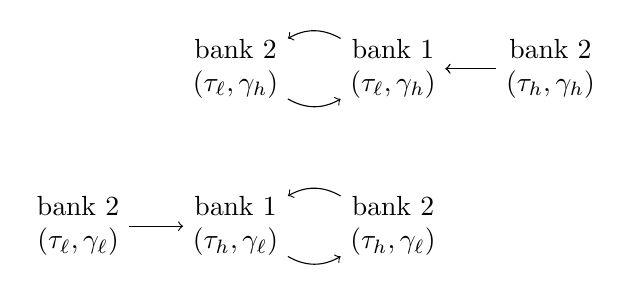
\begin{tikzpicture}
  % Nodes
    \node[align=center] (A) at (-2,0) {bank 2 \\ $(\tau_{\ell},\gamma_{\ell})$};
  \node[align=center] (B) at (0,0) {bank 1 \\ $(\tau_{h},\gamma_{\ell})$};
  \node[align=center] (C) at (2,0) {bank 2\\ $(\tau_{h},\gamma_{\ell})$};
  \node[align=center] (D) at (0,2) {bank 2\\ $(\tau_{\ell},\gamma_{h})$};
  \node[align=center] (E) at (2,2) {bank 1  \\ $(\tau_{\ell},\gamma_{h})$};
  \node[align=center] (F) at (4,2) {bank 2 \\ $(\tau_{h},\gamma_{h})$};
  % Arrows
  \draw[->] (A) -- (B);
  %\draw[->,red] (D) -- (E);
  %\draw[->,red] (C) -- (B);
  %\draw[->,red] (F) -- (C);
  \draw[->] (F) to (E);
  \draw[->,bend right] (B) to (C);
    \draw[->,bend right] (C) to (B);
     \draw[->,bend right] (D) to (E);
    \draw[->,bend right] (E) to (D);
    \draw[->] (F) to (E);
\end{tikzpicture} 
\caption{$\epsilon_1>0, \epsilon_2<0$.}
\end{minipage}
}
}
\caption{Alternative Best Response Dynamics. * The arrows means that, if bank 2 picks decision $(\tau_{\ell},\gamma_{\ell})$, the best response for Bank 1 is $(\tau_{h},\gamma_{\ell})$. ** The dashed arrow means that both case can happen, which depends on specific conditions on $D_y$. Note that it does not have an influence on the final conclusion, since both cases converge to the NE in the end. }
\label{fig:enter-label}
\end{figure}

% \subsection{Proof of Theorem \ref{thm:continous:peq}}
% \label{proof:continous}
% We first introduce the following simple lemma about the properties of $f$, which is easy to check.
% \begin{lemma}
% \label{lem:property of f}
% Assume $\emph{Supp}(D_y)=[0,1]$. We have
% \begin{enumerate}
%     \item $f(\gamma,\tau_a,\tau_b)$ is monotonically increasing with respect to $\gamma$. Moreover, let $y_{\gamma}=\frac{1}{2+\gamma}$, then $f(\gamma,y_{\gamma},\tau)$ is also monotonically increasing with respect to $\gamma$.
%     \item Let $\tau_a<\tau_b<\tau_c$. Then $f_{D_y}(\gamma_1,\tau_a,\tau_c)=f_{D_y}(\gamma_1,\tau_a,\tau_b)+f_{D_y}(\gamma_1,\tau_b,\tau_c)$.
%     \item Let $y_{\gamma}=\frac{1}{2+\gamma}$. If $y_{\gamma}\in(\tau_a,\tau_b)$, then $f(\gamma,\tau_a,y_{\gamma})<0$, and  $f(\gamma,y_{\gamma},\tau_b)>0$. 
% \end{enumerate}   
% \end{lemma}
% \noindent We analyze the existence of pure Nash equilibria under different conditions on the relationship between  decision pairs $\theta_1,\theta_2$. Firstly, note that, for a pair of $\theta_1,\theta_2$,  if the utility of a bank is strictly less than $0$, then the bank can always adjust its parameters $\gamma$ and $\tau$ to $1$ to ensure its utility becomes non-negative. This implies that decision pairs leading to non-positive utilities will not be an Nash equilibrium. Therefore, we only need to consider cases where $u_1 \geq 0$ and $u_2 \geq 0$.



% Next, we discuss the conditions for $\theta_1,\theta_2$ under which there are no pure NE under any distributions. We prove this by showing that, one can always find a new decision $\theta_1'=(\tau'_1,\gamma'_1)$ \textbf{or} $\theta_2'=(\tau'_2,\gamma'_2)$ for Bank 1 or 2 that leads to a larger utility for that bank.

% \paragraph{Case 1:} $\tau_1\leq \tau_2$, and $\gamma_1<\gamma_2$.
% In this case,   $u_1((\tau_1,\gamma_1),(\tau_2,\gamma_2))=f(\gamma_1,\tau_1,1),$ while $u_2=0.$ Let $\gamma_1'=\gamma_1+\epsilon<\gamma_2$ for some $\epsilon>0$. Then, $$u_1((\tau_1,\gamma_1'),(\tau_2,\gamma_2))=f(\gamma'_1,\tau_1,1)>f(\gamma_1,\tau_1,1)=u_1((\tau_1,\gamma_1),(\tau_2,\gamma_2)),$$ 
% where the inequality is based on the first property in Lemma \ref{lem:property of f}. It shows that $(\tau_1,\gamma_1')$ is a better decision for bank 1, therefor this case can not be a NE.   

% \paragraph{Case 2:} $\tau_1<\tau_2,\gamma_1=\gamma_2=\gamma$. In this case, $u_1((\tau_1,\gamma),(\tau_2,\gamma))=f(\gamma,\tau_1,\tau_2)+\frac{1}{2}f(\gamma,\tau_2,1)$, and $u_2((\tau_1,\gamma),(\tau_2,\gamma))=\frac{1}{2}f(\gamma,\tau_2,1)$. If $u_1((\tau_1,\gamma),(\tau_2,\gamma))=0,u_2((\tau_1,\gamma),(\tau_2,\gamma))>0$, then one can set $\tau_1'=\tau_2$, so that $$u_1((\tau_1',\gamma),(\tau_2,\gamma))=u_1((\tau_2,\gamma),(\tau_2,\gamma))=\frac{1}{2}f(\gamma,\tau_2,1)=u_2((\tau_1,\gamma),(\tau_2,\gamma))>0=u_1((\tau_1,\gamma),(\tau_2,\gamma)).$$
% If $u_1((\tau_1,\gamma),(\tau_2,\gamma))=u_2((\tau_1,\gamma),(\tau_2,\gamma))=0$, then it implies that $f(\gamma,\tau_1,\tau_2)=0$. Since $\text{Supp}(D_y)=[0,1]$, it means that there exists $\tau'\in(\tau_1,\tau_2)$ such that $f(\gamma,\tau_1,\tau')<0$ and $f(\gamma,\tau',\tau_2)>0$.  Therefore, if one sets $\tau_2'=\tau'$, we have 
% $$u_2((\tau_1,\gamma),(\tau'_2,\gamma))= f(\gamma,\tau',\tau_2)+\frac{1}{2}f(\gamma,\tau_2,1)>\frac{1}{2}f(\gamma,\tau_2,1)=u_2((\tau_1,\gamma),(\tau_2,\gamma)).$$
% \kri{Check these two subcases below, it's correct but I think some typo}
% If  $u_1((\tau_1,\gamma),(\tau_2,\gamma))>0$, $u_2((\tau_1,\gamma),(\tau_2,\gamma))=0$, it means that $f(\gamma,\tau_1,\tau_2)=0$. On the other hand, since $u_2=\frac{1}{2}f(\gamma,\tau_2,1)=\int_{\tau_2}^1[(2+\gamma)y-1]p(y)dy=0$, there exists a $\tau'\in(\tau_2,1)$, such that $(2+\gamma)\tau'-1=0$. Moreover, for all $\tau<\tau'$,  $(2+\gamma)\tau'-1<0$. This implies that $f(\gamma,\tau_1,\tau_2)<0$. This contradiction means that this case ($u_1((\tau_1,\gamma),(\tau_2,\gamma))>0$, $u_2((\tau_1,\gamma),(\tau_2,\gamma))=0$) will not happen. \\

% \noindent If $u_1((\tau_1,\gamma),(\tau_2,\gamma))>0$, and $u_2((\tau_1,\gamma),(\tau_2,\gamma))>0$, then let $y_{\gamma}=\frac{1}{2+\gamma}$. If $y_{\gamma}\in(\tau_1,\tau_2)$, then we have $f(\gamma,\tau_1,y_{\gamma})<0$, and $f(\gamma,y_{\gamma},\tau_2)>0$. Therefore, if one sets $\tau_1'=y_{\gamma}$, we have 
% $$u_1((\tau'_1,\gamma),(\tau_2,\gamma))=f(\gamma,y_{\gamma},\tau_2)>f(\gamma,\tau_1,y_{\gamma})+f(\gamma,y_{\gamma},\tau_2)=u_1((\tau_1,\gamma),(\tau_2,\gamma)).$$
% If $y_{\gamma}\geq \tau_2$, then we have $f(\gamma,\tau_1,\tau_2)< 0.$ Therefore, if we set $\tau_1'=\tau_2,$ we get 
% $$u_1((\tau_1',\gamma),(\tau_2,\gamma))=\frac{1}{2}f(\gamma,\tau_2,1)>f(\gamma,\tau_1,\tau_2)+\frac{1}{2}f(\gamma,\tau_2,1)>u_1((\tau_1,\gamma),(\tau_2,\gamma)).$$
% Similarly, if $y_{\gamma}\leq \tau_2$, setting $\tau_2'=\tau_1$ leads to a better utility for bank 2. 

% \paragraph{Case 3:} $\tau_1<\tau_2,$ $\gamma_1>\gamma_2$. In this case, $u_1((\tau_1,\gamma_1),(\tau_2,\gamma_2))=f(\gamma_1,\tau_1,\tau_2)$, and $u_2((\tau_1,\gamma),(\tau_2,\gamma))=f(\gamma_2,\tau_2,1)$. Let $y_{\gamma_{1}}=\frac{1}{2+\gamma_1}$, and $y_{\gamma_2}=\frac{1}{2+\gamma_2}$. Then, it is easy to check that if the pair of decisions will not be a NE if $\tau_1\not=y_{\gamma_{1}}$ or $\tau_2\not=y_{\gamma_{2}}$. \kri{We start by observing that for bank $2$ (with lower interest rate), it is optimal to set $\tau_2 = y_{\gamma_2}$ regardless of the other bank. Bank $2$ can always deviate to a threshold $y_{\gamma_2}$ and obtain higher utility, because if $y_{\gamma_2} < \tau_2$, it can drop threshold to $y_{\gamma_2}$ obtaining utility $f(\gamma_2, y_{\gamma_2}, 1) > f(\gamma_2, \tau_2, 1)$, similarly if $\tau_2 < y_{\gamma_2}$, bank 2 can increse threshold to $y_{\gamma_2}$ and get rid of the negative part of the integral}

% For example, if $\tau_1<y_{\gamma_{1}}$, then $f(\gamma_1,\tau_1,y_{\gamma_{1}})<0$, so setting $\tau_1'=y_{\gamma_{1}}$ leads to a larger utility for bank 1. For the case where $\tau_1=y_{\gamma_1}$ and $\tau_2=y_{\gamma_2}$, one can set $\gamma_2'=\gamma_2+\epsilon<\gamma_1$ for some $\epsilon>0$. In this case, 
% $$u_2((\tau_1,\gamma_1),(\tau_2,\gamma'_2))=f(\gamma_2',\tau_2,1)>f(\gamma_2,\tau_2,1)=u_2((\tau_1,\gamma_1),(\tau_2,\gamma_2)).$$


% Next, we discuss the case which can be a NE under certain conditions. 
% \paragraph{Case 4:} $\tau_1=\tau_2=\tau$, and $\gamma_1=\gamma_2=\gamma$. In this case, $u_1((\tau,\gamma),(\tau,\gamma))=u_2((\tau,\gamma),(\tau,\gamma))=\frac{1}{2}f(\gamma,\tau,1)$. Let $y_{\gamma}=\frac{1}{2+\gamma}$. If $y_{\gamma}>\tau$, then $f(\gamma,\tau,y)<0$, so if we sets $\tau'_2=y_{\gamma}$, we have 
% $$ u_2((\tau,\gamma),(\tau',\gamma))=\frac{1}{2}f(\gamma,y_{\gamma},1)>\frac{1}{2}f(\gamma,\tau,y_{\gamma})+\frac{1}{2}f(\gamma,y_{\gamma},1)=u_2((\tau,\gamma),(\tau,\gamma)).$$
% Similarly, if $y_{\gamma}<\tau$, we have $f(\gamma,y_{\gamma},\tau)>0$. Thus, we can set $\tau_2'=y_{\gamma}$, so 
% $$ u_2((\tau,\gamma),(\tau',\gamma))=\frac{1}{2}f(\gamma,y_{\gamma},1)>\frac{1}{2}f(\gamma,\tau,1)=u_2((\tau,\gamma),(\tau,\gamma)).$$
% The above discussion shows that this case will not be an NE if $\tau\not=y_{\gamma}.$ For the case where $\tau=y_{\gamma}$, we consider two possible situations: $\gamma>0$ and $\gamma=0$. If $\gamma>0$, then one can set $\gamma_1'=\gamma-\epsilon$ for a sufficiently small $\epsilon>0$, such that bank one double its profit with a very small cost (provided by $\epsilon$ is sufficiently small). If $\gamma=0$, then $\tau_1=\tau_2=y_{\gamma}=\frac{1}{2}$. In this case, no bank can double the profit by decreasing $\gamma$. Note that the game is symmetric, and the two players in this setting adopt the same decisions. Therefore, the decision pair $(\theta_1=(0.5,0),\theta_2=(0.5,0))$ will be an NE if and only if  
% $$u_1(\theta_1,\theta_2)\geq u_1(\theta'_1=(\tau',\gamma'),\theta_2),$$
% for any other $\theta_1'\in[0,1]^2$. If $\tau'>\tau$ and $\gamma'=\gamma$, then 
% $$u_1((\tau',\gamma'),\theta_2)=\frac{1}{2}f(\gamma,\tau',1)=\frac{1}{2}[f(\gamma,\tau,1) -f(\gamma,\tau,\tau')]<u_1(\theta_1,\theta_2),$$
% since $f(\gamma,\tau,\tau')>0$ by the definition of $y_{\gamma}.$
% If $\tau'<\tau$ and $\gamma'=\gamma$, then 
% $$u_1((\tau',\gamma'),(\tau,\gamma))=\frac{1}{2}f(\gamma,\tau',1)=\frac{1}{2}[f(\gamma,\tau'\tau)+f(\gamma,\tau,1)]<u_1(\theta_1,\theta_2),$$
% as $f(\gamma,\tau',\tau)<0.$ If $\tau'\geq\tau$ and $\gamma'>\gamma$, then $u_1((\tau',\gamma'),\theta_2)=0<u_1((\tau,\gamma),\theta_2)$. Finally, we consider the case where $\tau'<\tau$, and $\gamma'>\gamma$. In this case, 
% $$u_1((\tau',\gamma'),\theta_2)=\int^{\tau}_{\tau'}[(2+\gamma')y-1]p(y)dy.$$
% We have for all $(\tau',\gamma')$ such that $\tau'<\tau$ and $\gamma'>\gamma$, 
% $$\int^{\tau}_{\tau'}[(2+\gamma')y-1]p(y)dy\leq \int^{\tau}_{\tau'}[(2+1)y-1]p(y)dy\leq  \int^{\tau}_{y_1=\frac{1}{2+1}}[(2+1)y-1]p(y)dy=f\left(1,\frac{1}{3},0.5\right).$$
% This implies that, for all $(\tau',\gamma')$ such that $\tau'<\tau$ and $\gamma'>\gamma$, the maximum utility of bank 1 is achieved when $\tau'=\frac{1}{3}$, and $\gamma'=0.5$ \kri{$\gamma' = 1$ right?}. Therefore, $u_1(\theta_1,\theta_2)\geq u_1(\theta'_1=(\tau',\gamma'),\theta_2)$ if and only if 
% $$\frac{1}{2} f(0,0.5,1)\geq f\left(1,\frac{1}{3},0.5\right),$$
% \kri{Edited above}
% which finishes the proof. 



\subsection{Proof of Theorem \ref{thm:mixed-NE}}
\label{Proof:Theorem:mixedNE}
We overload notation and denote the expected utility of bank $i$ under $p_1$ and $p_2$ as:
$$ u_{i}(p_1,p_2)=\E_{\theta_1\sim p_1, \theta_2\sim p_2}[u_i(\theta_1,\theta_2)]. $$


\noindent Firstly, note that, based on Table \ref{tab:my-table} and Lemma \ref{lem:property of f}, it can be easily shown that for any $\theta\in\{\theta^{(j)}\}_{j=1}^4$, 
$$u_1(\theta^{(3)},\theta)> u_1(\theta^{(1)},\theta). $$
More specifically, 
\begin{equation*}
    \begin{split}
u_1(\theta^{(3)},\theta^{(1)})={} & \frac{1}{2}f(\gamma_{\ell},\tau_{h},1)>\frac{1}{2}f(\gamma_{\ell},\tau_{\ell},1) =   u_1(\theta^{(1)},\theta^{(1)}),\\
u_1(\theta^{(3)},\theta^{(2)})={} & f(\gamma_{\ell},\tau_{h},1)>f(\gamma_{\ell},\tau_{\ell},1) =   u_1(\theta^{(1)},\theta^{(2)}),\\
u_1(\theta^{(3)},\theta^{(3)})={} & \frac{1}{2}f(\gamma_{\ell},\tau_{h},1)>f(\gamma_{\ell},\tau_{\ell},\tau_h)+\frac{1}{2}f(\gamma_{\ell},\tau_h,1) =   u_1(\theta^{(1)},\theta^{(3)}),\\
u_1(\theta^{(3)},\theta^{(4)})={} & f(\gamma_{\ell},\tau_{h},1)>f(\gamma_{\ell},\tau_{\ell},1) =   u_1(\theta^{(1)},\theta^{(4)}),
    \end{split}
\end{equation*}
where the first, second and last inequality is because based on Lemma \ref{lem:property of f}, 
$$f(\gamma_{\ell},\tau_{\ell},1)=\underbrace{f(\gamma_{\ell},\tau_{\ell},\tau_{h})}_{<0}+f(\gamma_{\ell},\tau_{h},\tau_{h}),$$
and the third inequality is because $f(\gamma_{\ell},\tau_{\ell},\tau_{h})<0.$ This implies that $\theta^{(1)}$ is strictly dominated by $\theta^{(3)}$, and will not be part of the mixed NE. 


Since the game is symmetric, the same argument holds true for Bank 2, i.e. $u_2(\theta,\theta^{(3)}) > u_2(\theta,\theta^{(1)})$. By a similar argument, for any $\theta\in\{\theta^{(j)}\}_{j=2}^4$, we have
$$u_1(\theta^{(2)},\theta)> u_1(\theta^{(4)},\theta), $$
which indicates that $\theta^{(4)}$ will also not be part of mixed NE for Bank 1 or Bank 2.  To summarize, any mixed NE must satisfy $p_{1,1}=p_{1,4}=p_{2,1}=p_{2,4}=0$.\\


\noindent Consider a pair of mixed strategies $p_1=[0,p_{1,2},1-p_{1,2},0]$ and $p_2=[0,p_{2,2},1-p_{2,2},0]$. Then the utility of Bank 1 can be written as: 
\begin{equation}
    \begin{split}
    \label{eqn:u13123123}
u_{1}(p_1,p_2) = {} & \frac{1}{2} p_{1,2}p_{2,2} f(\gamma_{h}, \tau_{\ell}, 1) + p_{1,2}(1-p_{2,2})f(\gamma_{h},\tau_{\ell},\tau_{h})+ (1-p_{1,2})p_{2,2}f(\gamma_{\ell},\tau_h,1)\\
{} & + \frac{(1-p_{1,2})(1-p_{2,2})}{2}f(\gamma_{\ell},\tau_{h},1)\\       = {} & \frac{1}{2}p_{1,2}\left[(2-p_{2,2})f(\gamma_{h},\tau_{\ell},\tau_{h}) + p_{2,2}f(\gamma_{h},\tau_{h},1) -(1+p_{2,2})f(\gamma_{\ell},\tau_{h},1) \right] \\
{} & + \frac{(p_{2,2}+1)}{2}f(\gamma_{\ell},\tau_{h},1).
    \end{split}
\end{equation}
Note that it is a linear function with respect to $p_{1,2}$, and the slope is given by:
\begin{equation*}
    \begin{split}
        {} & \frac{1}{2} \left[(2-p_{2,2})f(\gamma_{h},\tau_{\ell},\tau_{h}) + p_{2,2}f(\gamma_{h},\tau_{h},1) -(1+p_{2,2})f(\gamma_{\ell},\tau_{h},1)\right]\\
        = {} & \frac{1}{2} p_{2,2}[f(\gamma_{h},\tau_{h},1)-f(\gamma_{\ell},\tau_{h},1)-f(\gamma_{h},\tau_{\ell},\tau_{h})] + f(\gamma_{h},\tau_{\ell},\tau_{h}) - \frac{1}{2} f(\gamma_{\ell},\tau_{h},1),
    \end{split}
\end{equation*}
Let 
\begin{equation}
\label{eqn:def-of-g(p)}
g(p)=p[f(\gamma_{h},\tau_{h},1)-f(\gamma_{\ell},\tau_{h},1)-f(\gamma_{h},\tau_{\ell},\tau_{h})] + 2f(\gamma_{h},\tau_{\ell},\tau_{h}) - f(\gamma_{\ell},\tau_{h},1).
\end{equation}
Then, the slope of $u(p_1,p_2)$ with respect to $p_{1,2}$ is given by $\frac{1}{2} g(p_{2,2})$.
Moreover, (recalling our definitions of the shorthand notation $\epsilon_1 = \frac{1}{2} f(\gamma_h, \tau_{\ell},1) - f(\gamma_{\ell},\tau_h, 1)$ and $\epsilon_2 = f(\gamma_h, \tau_{\ell}, \tau_h) - \frac{1}{2} f(\gamma_{\ell},\tau_h, 1)$), we note that $g(p):[0,1]\mapsto \R$ is a linear function, $g(0)=2\epsilon_2$, and $g(1)=2\epsilon_1$.
\\
\noindent 

Let $BR_1(p) \subseteq [0,1]$ denote the candidate set of best response probabilities of picking $\theta^{(2)}$ of Bank 1 if Bank 2 picks $p_2=[0,p,1-p,0]$. 
The corresponding candidate set for Bank 2 is denoted by $BR_2(p)$.

Then, consider the following cases: 

\noindent \paragraph{Case 1:} $\epsilon_1<0$, $\epsilon_2<0$. Therefore, $g(0)=2\epsilon_2<0$ and  $g(1)=2\epsilon_1<0$, 
then it is clear that $g(p)<0$ for all $p\in[0,1]$. 
This means that the slope in \eqref{eqn:u13123123} will always be negative, so $BR_1(p)= \{0\}$ for any $p\in[0,1]$. Similarly, $BR_2(p)=\{0\}$ for any $p\in[0,1]$, which indicates that $p_{1,2}=p_{2,2}=0$, $p_{1,3}=p_{2,3}=1$ is the only mixed NE (and, in fact, this corresponds to a pure NE).

\noindent \paragraph{Case 2:} $\epsilon_1<0$, $\epsilon_2>0$. Therefore, $g(0)>0$, and $g(1)<0$, and since $g$ is a linear function, it means that there must exist a unique $c\in(0,1)$, such that $g(c)=0$. Based on \eqref{eqn:def-of-g(p)}, we know 
$$ c=\frac{f(\gamma_{\ell},\tau_h,1)-2f(\gamma_h,\tau_{\ell},\tau_h)}{f(\gamma_h,\tau_h,1)-f(\gamma_{\ell},\tau_h,1)-f(\gamma_h,\tau_{\ell},\tau_h)}.$$
Combining with \eqref{eqn:u13123123}, we have 
\begin{equation*}
BR_1(p)= 
    \begin{cases}
        \{0\}, & p>c;\\
        \{1\},  & p<c;\\
        [0,1], & p=c.
    \end{cases}
\end{equation*}
This is because, if $p>c$, $g(p)<0$, so the slope in \eqref{eqn:u13123123} is negative, and $BR_1(p)=\{0\}$.If $p<c$, then $g(p)>0$, the slope in \eqref{eqn:u13123123} is positive, and $BR_1(p)=\{1\}$. If $p=c$, \eqref{eqn:u13123123} will not be a function of $p_{1,2}$, so any decision for Bank 1 leads to the same gain. Similarly, we have 
\begin{equation*}
BR_2(p)= 
    \begin{cases}
        \{0\}, & p>c;\\
        \{1\},  & p<c;\\
        [0,1], & p=c.
    \end{cases}
\end{equation*}
Therefore, we know that $([0,c,1-c,0],[0,c,1-c,0])$ is a mixed NE, and $([0,0,1,0],[0,1,0,0])$ and $([0,1,0,0],[0,0,1,0])$ are also pure NEs. 

\noindent \paragraph{Case 3:} $\epsilon_1>0$, $\epsilon_2<0$. Therefore, $g(0)<0$, and $g(1)>0$, and since $g$ is a linear function, it means that there must exist $c\in(0,1)$, such that $g(c)=0$. 
Combining with \eqref{eqn:u13123123}, we have 
\begin{equation*}
BR_1(p)= 
    \begin{cases}
        \{1\}, & p>c;\\
        \{0\},  & p<c;\\
        [0,1], & p=c.
    \end{cases}
\end{equation*}
Similarly, we have 
\begin{equation*}
BR_2(p)= 
    \begin{cases}
        \{1\}, & p>c;\\
        \{0\},  & p<c;\\
        [0,1], & p=c.
    \end{cases}
\end{equation*}
Therefore, we know that $([0,c,1-c,0],[0,c,1-c,0])$ is a mixed NE, and $([0,0,1,0],[0,0,1,0])$ and $([0,1,0,0],[0,1,0,0])$ are also pure NEs. 

\noindent \paragraph{Case 4:} $\epsilon_1>0$, $\epsilon_2>0$. In this case, we know that $g(p)>0$ for all $p\in[0,1]$. Then, we have $BR_1(p)=\{1\}$, and $BR_2(p)=\{1\}$, which implies that the only mixed NE here is $([0,1,0,0], [0,1,0,0])$ (which is in fact a pure NE).
This completes the proof of the theorem.

\subsection{Proof of Theorem \ref{thm:cE}}
\label{proof:CE}

Firstly, we know $u_i(\theta^{(3)},\theta)> u_i(\theta^{(1)},\theta),$. This means $\theta^{(1)}$ will not be part of CE. Conditioned on this, for any $\theta\in\{\theta^{(j)}\}_{j=2}^4$, we have
$u_1(\theta^{(2)},\theta)> u_1(\theta^{(4)},\theta).$ This indicates that $\theta^{(4)}$ will no be part of CE. Thus, $p_{11}=\dots,=p_{14}=0$, $p_{11}=\dots,=p_{41}=0$, $p_{14}=\dots,=p_{44}=0$, $p_{41}=\dots,=p_{44}=0$. Next, based on Definition \ref{defn:CE}, we firstly need:
\begin{equation*}
    \begin{split}
     \sum_{i=2}^3 u_1\left((\tau_{\ell},\gamma_{h}),\theta^{(i)}\right)p_{2i} \geq {} &    \sum_{i=2}^3 u_1\left(\theta',\theta^{(i)}\right)p_{2i},\ \forall \theta'\in\Theta, 
    \end{split}
\end{equation*}
That is, for $\theta'=\theta^{(1)}$,
\begin{equation*}
    \begin{split}
 p_{22}\frac{1}{2}f(\gamma_h,\tau_{\ell},1) + p_{23} f(\gamma_h,\tau_{\ell},\tau_{h}) \geq  p_{22} f(\gamma_{\ell},\tau_{\ell},1) + p_{23} (f(\gamma_{\ell},\tau_{\ell},\tau_h)+\frac{1}{2}f(\gamma_{\ell},\tau_h,1)),     
    \end{split}
\end{equation*}
that is, 
$$ p_{22}(\epsilon_1-f(\gamma_{\ell},\tau_{\ell},\tau_h) )\geq p_{23}(f(\gamma_{\ell},\tau_{\ell},\tau_h)-\epsilon_2  ),$$
that is 
\begin{equation}
\label{eqn:ce:drop1}
    p_{22}\epsilon_1 \geq -p_{23}\epsilon_2 + (p_{22}+p_{23})f(\gamma_{\ell},\tau_{\ell},\tau_h). 
\end{equation}
For $\theta'=\theta^{(3)}$, we have 
\begin{equation}
\label{eqn:ce:nodrop1}
     p_{22}\epsilon_1 \geq  -p_{23}\epsilon_2.
\end{equation}
Note that since 
$f(\gamma_{\ell},\tau_{\ell},\tau_h)$ is negative, we know that \eqref{eqn:ce:nodrop1} implies \eqref{eqn:ce:drop1}, and thus \eqref{eqn:ce:drop1} can be dropped. 

For $\theta'=\theta^{(4)}$, we have 
\begin{equation*}
    \begin{split}
 p_{22}\frac{1}{2}f(\gamma_h,\tau_{\ell},1) + p_{23} f(\gamma_h,\tau_{\ell},\tau_{h}) \geq  p_{22} \frac{1}{2}f(\gamma_{h},\tau_h,1) + p_{23} 0,     
    \end{split}
\end{equation*}
which always holds true. Next, we need 
\begin{equation*}
    \begin{split}
     \sum_{i=2}^3 u_1\left((\tau_{h},\gamma_{\ell}),\theta^{(i)}\right)p_{3i} \geq {} &    \sum_{i=2}^3 u_1\left(\theta',\theta^{(i)}\right)p_{3i},\ \forall \theta'\in\Theta. 
    \end{split}
\end{equation*}
For $\theta'=\theta^{(1)}$, it means 
$$p_{32} f(\gamma_{\ell},\tau_{h},1) + p_{33}\frac{1}{2}f(\gamma_{\ell},\tau_h,1)\geq p_{32} f(\gamma_{\ell},\tau_{\ell},1) + p_{33} \left(f(\gamma_{\ell},\tau_{\ell},\tau_h)+\frac{1}{2}f(\gamma_{\ell},\tau_h,1)\right), $$
which always holds true. For $\theta'=\theta^{(2)}$, we have 
$$ -p_{32}\epsilon_1\geq p_{33}\epsilon_2.$$
For $\theta'=\theta^{(4)}$, we have 
$$ p_{32} f(\gamma_{\ell},\tau_{h},1) + p_{33}\frac{1}{2}f(\gamma_{\ell},\tau_h,1) \geq p_{32} \frac{1}{2} f(\gamma_{h},\tau_h,1). $$
Rearrange, we have
$$ -p_{32}\epsilon_1\geq p_{33}\epsilon_2 -\left(p_{33}+\frac{1}{2}p_{32}\right)f(\gamma_{h},\tau_{\ell},\tau_h). $$
Since $f(\gamma_{h},\tau_{\ell},\tau_h)$ is positive, the above condition is implied by $ -p_{32}\epsilon_1\geq p_{33}\epsilon_2,$ and thus can be dropped. 

To proceed, we need 
\begin{equation*}
    \begin{split}
     \sum_{i=2}^3 u_2\left(\theta^{(i)},(\tau_{\ell},\gamma_{h})\right)p_{i2} \geq {} &    \sum_{i=2}^3 u_2\left(\theta^{(i)},\theta'\right)p_{i2},\ \forall \theta'\in\Theta, 
    \end{split}
\end{equation*}
which is equivalent to 
\begin{equation*}
    \begin{split}
     \sum_{i=2}^3 u_1\left((\tau_{\ell},\gamma_{h}),\theta^{(i)}\right)p_{i2} \geq {} &    \sum_{i=2}^3 u_1\left(\theta',\theta^{(i)}\right)p_{i2},\ \forall \theta'\in\Theta. 
    \end{split}
\end{equation*}
Thus, following similar procedure, the condition we get is 
$$ p_{22}\epsilon_1\geq -p_{32}\epsilon_2. $$
Finally, for 
\begin{equation*}
    \begin{split}
     \sum_{i=2}^3 u_2\left(\theta^{(i)},(\tau_{h},\gamma_{\ell})\right)p_{i3} \geq {} &    \sum_{i=2}^3 u_2\left(\theta^{(i)},\theta'\right)p_{i3},\ \forall \theta'\in\Theta, 
    \end{split}
\end{equation*}
we get 
$$ -p_{23}\epsilon_1\geq p_{33}\epsilon_2,$$
To summarize, we have the following conditions:
\begin{align}
        p_{22}\epsilon_1 \geq {} & -p_{23}\epsilon_2 \label{eq:first}\\
        -p_{32}\epsilon_1\geq {} & p_{33}\epsilon_2 \label{eq:second}.\\
        p_{22}\epsilon_1\geq {} & -p_{32}\epsilon_2 \label{eq:fourth}\\
         -p_{23}\epsilon_1\geq {} & p_{33}\epsilon_2 \label{eq:fifth},
\end{align}
When $\epsilon_1>0$ and $\epsilon_2>0$, from \eqref{eq:second} and \eqref{eq:fifth}, we know that $p_{32}=p_{33}=p_{23}=0$, which leads to $p_{22}=1$, and it can make sure all inequality is ture. Similarly,  when $\epsilon_1<0$ and $\epsilon_2<0$, we get $p_{22}=p_{32}=p_{23}=0$, and $p_{33}=1$.

When $\epsilon_1>0,\epsilon_2<0$,  we need $\min\{p_{22},p_{33}\}>\max\left\{ \frac{|\epsilon_2|}{\epsilon_1}p_{23}, \frac{\epsilon_1}{|\epsilon_2|}p_{32} \right\}$. For  $\epsilon_1<0$ and $\epsilon_2>0$, we need $\min\{p_{23},p_{32}\}>\max\left\{ \frac{|\epsilon_1|}{\epsilon_2}p_{22}, \frac{\epsilon_2}{|\epsilon_1|}p_{33} \right\}$. 
